CMake is open source and available on many platforms. It is also compiler-independent, making it a very strong tool when it comes to building and distributing cross-platform software. All these features make it a valuable tool for building software in a modern way – that is, by relying heavily on build automation and built-in quality gates.

CMake consists of three command-line tools:

\begin{itemize}
\item 
cmake: CMake itself, which is used to generate build instructions

\item 
ctest: CMake's test utility, which is used to detect and run tests

\item 
cpack: CMake's packaging tool, which is used to pack software into convenient installers, such as deb, RPM, and self-extracting installers
\end{itemize}

There are also two interactive tools:

\begin{itemize}
\item 
cmake-gui: A GUI frontend to help with configuring projects

\item 
ccmake: An interactive terminal UI for configuring CMake
\end{itemize}

cmake-gui can be used to conveniently configure a CMake build and select the compiler to be used:

\begin{center}
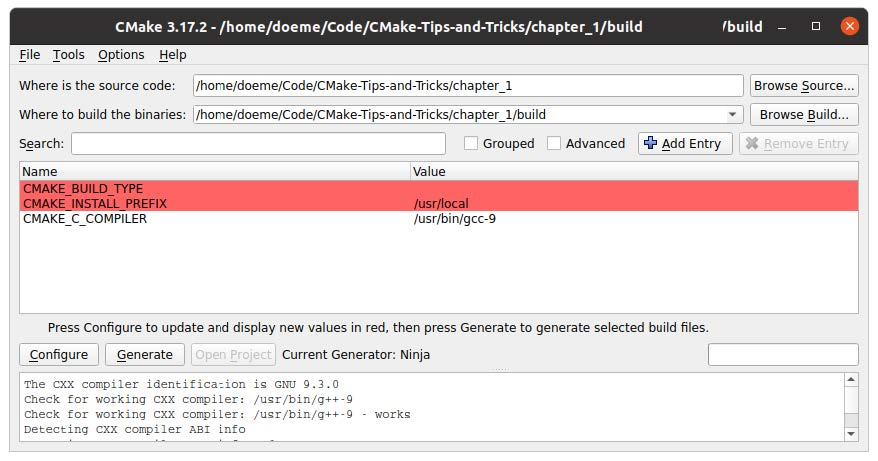
\includegraphics[width=1.\textwidth]{content/1/chapter1/images/1.jpg}\\
Figure 1.1 – cmake-gui after configuring a project
\end{center}

If you're working on the console but still want to have an interactive configuration of CMake, then ccmake is the right tool. While not as convenient as cmake-gui, it offers the same functionality. This is especially useful when you must configure CMake remotely over an ssh shell or similar:

\begin{center}
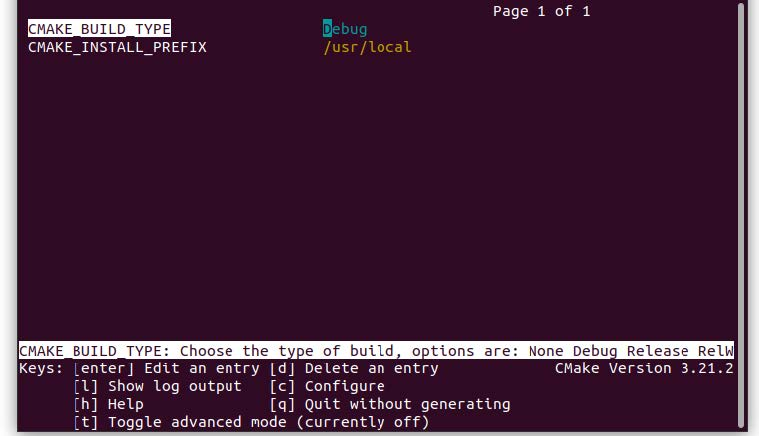
\includegraphics[width=1.\textwidth]{content/1/chapter1/images/2.jpg}\\
Figure 1.2 – Configuring a project using ccmake
\end{center}

The advantage of CMake over a regular build system is manyfold. First, there is the cross-platform aspect. With CMake, it is much easier to create build instructions for a variety of compilers and platforms without the need to know the specifics of the respective build system in depth.

Then, there is CMake's ability to discover system libraries and dependencies, which lessens the pain of locating the correct libraries for building a piece of software considerably. An additional bonus is that CMake integrates nicely with package managers such as Conan and vcpkg.

It is not just the ability to build software for multiple platforms, but also its native support for testing, installing, and packaging software that makes CMake a much better candidate for building software than just a single build system. Being able to define everything from building and over-testing to packaging at a single point helps tremendously with maintaining projects in the long run.

The fact that CMake itself has very few dependencies on the system and can run on the command line without user interaction makes it very suitable for build system automatization in CI/CD pipelines.

Now that we've covered briefly what CMake can do, let's learn how to install CMake.






















